\documentclass[a4paper,10pt]{article}

\usepackage{graphicx}
\usepackage{listings}
\usepackage{hyperref}

\usepackage[ansinew]{inputenc}
\usepackage[spanish]{babel}

\title{
    \textbf{TP0 - Mandelbrot}
}

\author{
    Juan Facundo Tkaczyszyn , \textit{Padr�n Nro. 87.931}                 \\
    \texttt{ facu.tk@gmail.com }                                          \\[2.5ex]
    Santiago Weber, \textit{Padr�n Nro. 00.000}                           \\
    \texttt{ santiago.weber91@gmail.com }                                 \\[2.5ex]
    \normalsize{2do. Cuatrimestre de 2014}                                \\
    \normalsize{66.20 Organizaci�n de Computadoras  $-$ Pr�ctica Martes}  \\
    \normalsize{Facultad de Ingenier�a, Universidad de Buenos Aires}      \\
}

\date{}

\begin{document}

\maketitle
\thispagestyle{empty}   % quita el n�mero en la primer p�gina


\begin{abstract}
El set de Mandelbrot es un \textit{fractal}. A lo largo de este trabajo pr�ctico lo
analizamos, y construimos un programa que permite dibujarlo centrado y acercado
a donde se le indique.
Este informe refleja las consideraciones que tomamos al encarar el trabajo
pr�ctico, las pruebas y el c�digo fuente entregable.
\end{abstract}


\pagebreak

\tableofcontents
\thispagestyle{empty}   % quita el n�mero en esta p�gina
\pagebreak

\section{Introducci�n}
\subsection{N�mero Complejo}

Un n�mero complejo\cite{CMPLX} es un n�mero, pero diferente de los n�mero normales.  \\
Se puede representar juntado dos n�meros.\\
La primera parte es un n�mero real. La segunda parte de un n�mero complejo es un n�mero \textit{imaginario}\cite{IMAGN}. \\
\\
La parte mas importante del n�mero imaginario se la conoce como i, definida como $\sqrt{-1}$. Todos los demas n�meros imaginarios son el n�mero i multiplicado por un n�mero real. \\
\\
Al n�mero complejo lo podemos escribir como a+bi, siendo a y b n�meros reales. \\
Dado que este n�mero tiene dos componentes, la real y la imaginaria, podemos usar esas componentes para representarlo en un sistema de coordenadas Cartesianadas.  \\
Esta representaci�n la conocemos como plano complejo.

\subsection{Mandelbrot}

El set de Mandelbrot\cite{MNDL1}\cite{MNDL2} es un fractal.  \\
\\
Empieza con la ecuaci�n: \\
%\\
\begin{center}
$Z_{n+1} = Z^{2}_n + c$
\end{center}
%\\
Donde c y z son n�mero complejos y n es cero o un n�mero entero positivo. \\
\\
Empezando en $z_0 = 0$, c esta en el set de Mandelbrot si el valor absoluto de $Z_n$ nunca excede cierto n�mero. \\
\\
Tomando por ejemplo, c = 1+0i. La secuencia es 0, 1, 2, 5, 26... que se va a inf�nito. Por lo tanto 1+0i no pertenece al conjunto. \\
Por otro lado, si tomamos c = 0+1i, la secuencia es 0, i, (-1 + i), -i, (-1 + i), -i, que no se va al infinito, entonces pertenece al conjunto de mandelbrot.  \\
La intensidad del color estada dada por la cantidad de iteraciones que tiene que hacer el algoritmo hasta exceda el valor absoluto, o se alcanze una cantidad maxima de iteraciones.  \\

\pagebreak

\section{An�lisis}

\subsection{Interfaz}

El programa tiene que ser capaz de leer argumentos pasados por linea de comandos.  \\
\\
Para parametros como la resolucion ( ej: 640x480 ), o el centro ( ej: 1-4.5i), debe validar que se cumpla con el formato correcto y se traiga el tipo de dato correcto.

\subsection{Salida}

\subsubsection{Archivo/Salida Standard}

El programa toma el parametro de entrada y debe decidir si tiene que salir a un archivo, o salir por salida standard\cite{STDOU}. \\
En caso que salga por un archivo debe validar que sea posible la escritura al mismo.

\subsubsection{Formato PGM}

El formato PGM\cite{PGM01} es una formato para almacenar informacion grafica en un texto plano.  \\
\\
Se detalla abajo un ejemplo de un cuadrado negro sobre un fondo blanco.

\begin{lstlisting}[
    language=bash,
    basicstyle=\small\ttfamily
]

    P2              #Header
    4               # Cantidad de filas
    4               # Cantidad de columnas
    255             # Maximo valor que puede tener un punto
    255 225 255 255 # Matriz de puntos
    255   0   0 255 
    255   0   0 255 
    255 225 255 255 

\end{lstlisting}

\pagebreak

\section{Dise�o}
\subsection{Consideraciones}
El primer paso de este desarrollo fue el de discretizar el centro y ventana pedidas a una cantidad de punto finita en el plano complejo.  \\
Buscando un poco, encontramos un ejemplo sobre el cual nos basamos en Rossetta Code\cite{MNDLC}.\\
\\
Para tomar los parametros que el usuario le pasa a nuestro programa por consola utilizamos getopt\_long\cite{GETOP}.  \\
Luego, para validar que los argumentos pasados cumplan con los formatos esperados usamos sscanf\cite{SSCAN}.  \\
Finalmente, para cada punto procesado que debemos escribir a un archivo, utilizamos fwrite\cite{FWRIT},
ya que su interfaz pide un identificador de archivo y el texto que vamos a escribir.
Esto nos permite usar la misma funcion si estamos escribiendo a un archivo o a salida standard.\\
\\
El modulo donde calculamos los valores para los puntos y escribimos a un archivo
nos planteo un problema de dise�o. Lo escribimos de forma tal que no instanciara
memoria, simplemente discretiza los puntos, calcula la intensidad para cada
punto y lo escribe a al archivo.\\
Este enfoque no era testeable.  \\
\\
Una alternativa era separar la funcionalidad de discretizacion y calculo, de la de escritura al archivo.  \\
\\
La alternativa por la que optamos fue aplicar Inversion de
dependencias\cite{DIP} en el modulo que discretiza, calcula y escribe, pasandole
por parametro cual es la funcion que debe usar a la hora de escribir.
De esta forma, al compilarlo para la entrega se utiliza la funcion fwrite. Pero
cuando se compila para pruebas se utiliza una funcion fwrite propia, con la
misma firma, pero que en vez de escribir al archivo, escribe a un buffer interno
contra el cual despues comparamos los resultados esperados.

\pagebreak

\section{Construcci�n}
\subsection{Makefile}
Como primer paso para asegurarnos que siempre se va a compilar igual, usando las
mismas fuentes, con los mismos niveles de optimizacion en las diferentes
plataformas donde desarrollaramos y testearamos, escribimos un
Makefile\cite{MAKE} con tres targets: all, tests y clean.
\\
all compila el codigo para la entrega, tests compila y corre las pruebas
unitarias, clean borra los ejecutables compilados.

\subsection{Pruebas Unitarias}
Para validar todos los requisitos funcionales escribimos pruebas unitarias.  \\
Como framework de pruebas utilizamos CuTest\cite{CUTST} por su portabilidad al
Netbsd de pruebas. \\
\\
Detallamos las firmas de algunas de las pruebas que escribimos para validar los
requisitos. Como el codigo de estas pruebas escapa al alcance de la entrega no
lo incluimos en el codigo impreso, pero se encuentra disponible en el repositorio\cite{REPO}.  \\
\begin{lstlisting}[
    language=c,
    basicstyle=\small\ttfamily
]

    /*
     *  --width w
     */
        // Si le pasamos 10, esperamos 10
        test_parse_width_gets_10_returns_10

        // Si le pasamos una A, esperamos un error
        test_parse_width_gets_A_halts

        // Si le pasamos un ancho negativo, esperamos un error
        test_parse_width_gets_negative_halts

    /*
     *  --resolution rx_ry
     */
        // Si le pasamos una resolucion 16x12, esperamos 16x12
        test_parse_resolution_gets_16x12_returns_16x12

        // Si algun componente es negativo, esperamos error
        test_parse_resolution_gets_negative_halts

    /*
     *  --center a+bi
     */
        // Si se invoca al parametro pero vuelve vacio, esperamos error
        test_parse_center_gets_empty_halts

        // Si le pasamos 1-2i, esperamos 1-2i
        test_parse_center_gets_1_2i_neg_returns_1_2i_neg

\end{lstlisting}

\pagebreak

\section{Pruebas}

\subsection{Corridas de prueba}

Documentamos tres corridas de prueba. Definimos centro y tama�o de ventana y
generamos una salida por consola con baja resoluci�n, y luego una con mayor
resoluci�n que convertimos en gr�fico.


\subsection{Centrado en 0, ventana de 2}

\begin{lstlisting}[
    language=bash,
    basicstyle=\small\ttfamily
]
    $ ./tp0 --center 0+0i --width 2 --height 2
            --resolution 14x11 --output -

    P2
    14
    11
    255
      2   2   2   3   3   4  12  44   3   2   2   1   1   1 
      2   3   3   3   5   9 255  24   4   3   3   2   1   1 
      3   4   5  65  10 255 255 255  30   8   5   2   2   1 
      4   5   8 239 255 255 255 255 255 255   6   3   2   2 
    255  12  52 255 255 255 255 255 255 255   8   3   2   2 
    255 255 255 255 255 255 255 255 255 255   5   3   2   2 
    255 255 255 255 255 255 255 255 255  14   5   3   2   2 
    255  12  52 255 255 255 255 255 255 255   8   3   2   2 
      4   5   8 239 255 255 255 255 255 255   6   3   2   2 
      3   4   5  65  10 255 255 255  30   8   5   2   2   1 
      2   3   3   3   5   9 255  24   4   3   3   2   1   1 

\end{lstlisting}

\begin{figure}[!htp]
\begin{center}

\includegraphics[width=0.7\textwidth]{images/mandelbrot_0.eps}
\caption{ Mandelbrot0 }
\label{mandelbrot_0}
\end{center}
\end{figure}

\pagebreak


\subsection{Centrado en -0.165+1.039i, ventana de 0.006}
\begin{lstlisting}[
    language=bash,
    basicstyle=\small\ttfamily
]
    $ ./tp0 --width 0.006089755361389781 --height 0.006089755361389781
            --center -0.16495019360389762+1.0391402340922113i
            --resolution 14x11 --output -

    P2
    14
    11
    255
     26  32  26  31  24  22  21  21  23  25  22  21  22  26 
     47  34  41  29  25  29  24  24  26  29  24  34  25  30 
     30  54  49  34  31  30  27  26  31  28  27  29  34  58 
     27  32  35  56  41  35  36  34  36  32  36  34  72  44 
     22  30  39  33  40  81  45  45  53  45  49  43  55  96 
     22  24  26  32  37  55 127 119 123  63  69 103 117 255 
     39  29  28  30  37  47  84 255 255 255 255 255 255 255 
     22  24  27  30  52  41 103  86 255 255 255 255 255 255 
     21  22  24  27  35  39  78 105 255 255 255 255 255 255 
     21  23  31  30  34  40  50 255 255 255 255 255 255 255 
     23  24  26  32  52  61  76 255 255 255 255 255 255 255 

\end{lstlisting}

\begin{figure}[!htp]
\begin{center}

\includegraphics[width=0.7\textwidth]{images/mandelbrot_1.eps}
\caption{ Mandelbrot1 }
\label{mandelbrot_1}
\end{center}
\end{figure}

\pagebreak



\subsection{Centrado en -0.027+0.709i, ventana de 0.009}

\begin{lstlisting}[
    language=bash,
    basicstyle=\small\ttfamily
]
    $ ./tp0 --width 0.00913463304208467 --height 0.00913463304208467
            --center -0.027010582808902495+0.7093001367538602i
            --resolution 14x11 -output -

    P2
    14
    11
    255
    255 255 255 255 255 255 107  84  88  52  39  36  39  64 
    255 255 255 255 255 255  86 125  61  47  40  39  66  52 
    255 255 255 255 255 255 255  63  59  64  42  42  44  63 
    255 255 255 255 255 255 228 255 230  53  45  44  45  46 
    255 255 255 255 255 255 255 202 140  54 110  85  49  52 
    255 255 255 255 255 255 255 179  74  61  58  64  81  90 
    255 255 255 224 255 255 164 139 105  85 100 196 105 117 
    255 149 217 144  73 230 158  71 154 175  92  75  62  49 
    255  90  78  58  53  56  81  58  81  74  97  93 115  61 
    194 255 255 118  48  43  45  49  70  66  97  83  49  55 
     58  64  84  72  47  48  38  55  52  45  43 123  38  34 

\end{lstlisting}

\begin{figure}[!htp]
\begin{center}
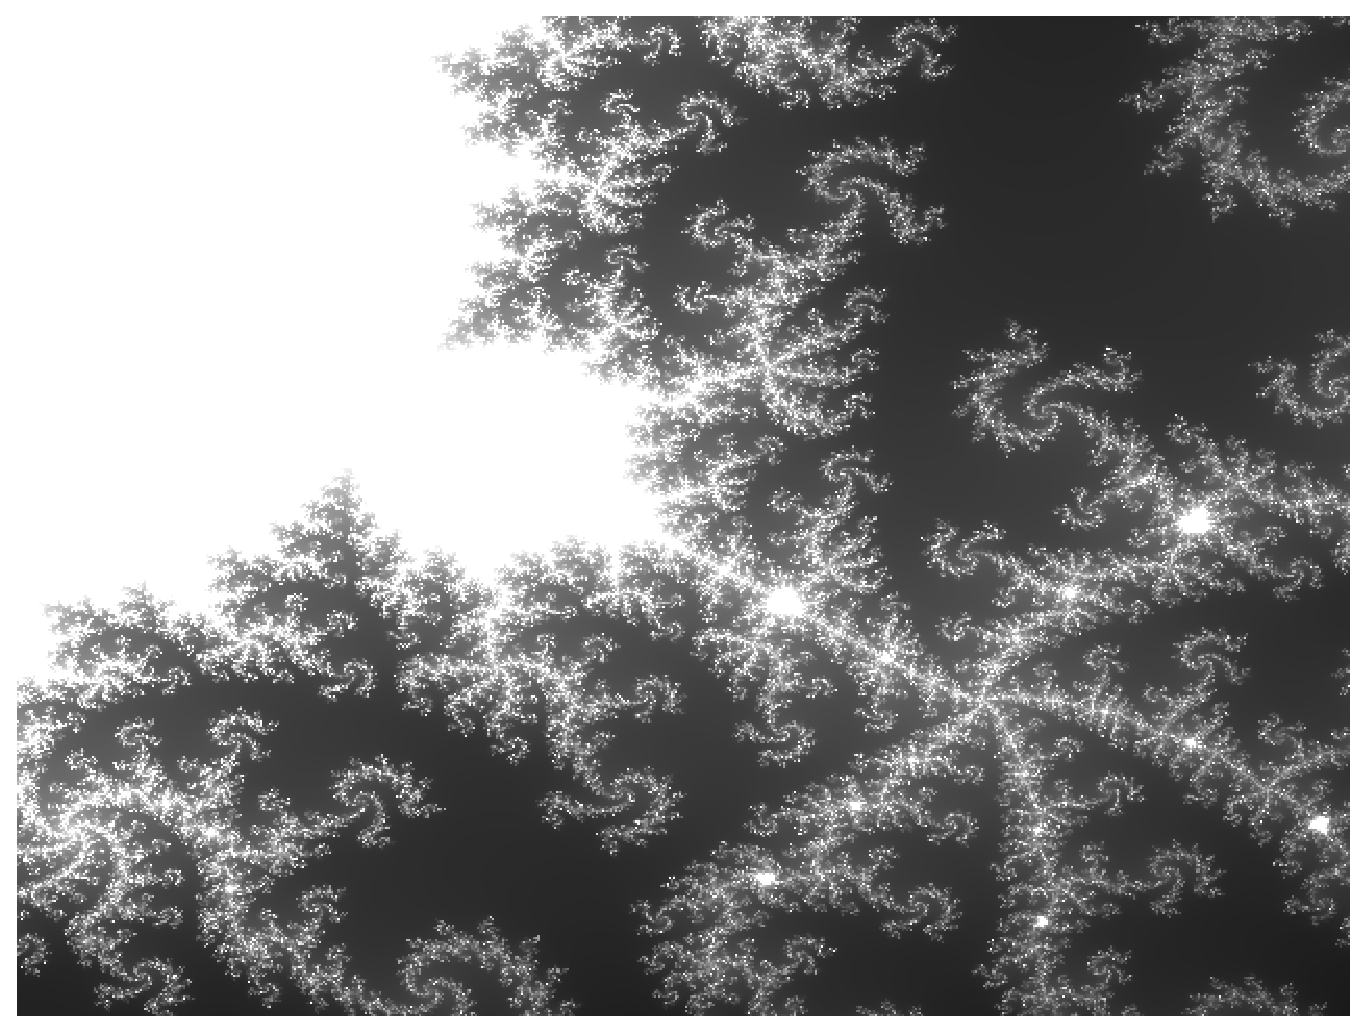
\includegraphics[width=0.7\textwidth]{images/mandelbrot_2.eps}
\caption{ Mandelbrot2 }
\label{mandelbrot_2}
\end{center}
\end{figure}

\pagebreak

\subsection{Pruebas Unitarias}

Para correr las pruebas unitarias, invocamos al target test de nuestro makefile.  Abajo exponemos el resultado de dicha corrida.

\begin{lstlisting}[
    language=bash,
    basicstyle=\small\ttfamily
]

    make tests

    ./tests
    .....................

    OK (21 tests)


\end{lstlisting}

\subsection{Emulador MIPS}

Para correr las pruebas sobre el NetBSD\cite{NTBSD}, corremos el
GXemul\cite{GXEML} tal como se nos explico en clase y luego copiamos la carpeta
mediante SSH\cite{SSH}, con el comando SCP. Navegamos hasta la carpeta del
makefile y escribimos.

\begin{lstlisting}[
    language=bash,
    basicstyle=\small\ttfamily
]

    make tests

\end{lstlisting}

\pagebreak

\section{C�digo Fuente}

Se expone el c�digo fuente del programa. El c�digo fuente de las pruebas unitarias se encuentra en el repositorio\cite{REPO}\\

\subsection{default\_values.h}
\lstinputlisting[ language=c, basicstyle=\small\ttfamily ]{../src/default_values.h}

\pagebreak

\subsection{main.c}
\lstinputlisting[ language=c, basicstyle=\small\ttfamily ]{../src/main.c}
\pagebreak

\subsection{mandelbrot.c}
\lstinputlisting[ language=c, basicstyle=\small\ttfamily ]{../src/mandelbrot.c}
\pagebreak

\subsection{parse\_opt.c}
\lstinputlisting[ language=c, basicstyle=\small\ttfamily ]{../src/parse_opt.c}
\pagebreak


\section{Extras}

\subsection{Render Online}

Luego que concluimos con la construcci�n y las pruebas, fuimos un paso mas y
desarrollamos una interfaz para tomar parametros via web, y la matriz de salida
generada convertirla en una imagen. Se encuentra disponible en
\href{http://home.facu.tk/mandelbrot}{http://home.facu.tk/mandelbrot}
y el c�digo en la carpeta del repositorio\cite{REPO}.\\

\subsubsection{Flask}

Desarrollamos un wrapper en Python\cite{PYTHN} para tomar los parametros de un query
string HTTP, y mapearlos a un comando de linea de comandos.

\begin{lstlisting}[ language=bash, basicstyle=\small\ttfamily ]
    http://SERVER/?opcion=argumento
\end{lstlisting}

lo mapeamos a:

\begin{lstlisting}[ language=bash, basicstyle=\small\ttfamily ]
    ./tp0 -opcion argumento
\end{lstlisting}

Para la parte web utilizamos Flask\cite{FLASK}, un framework de desarrollo web liviano escrito en Python.

Se detalla abajo la parte relevante del c�digo.

\begin{lstlisting}[
        language=python,
        basicstyle=\small\ttfamily 
                  ]

    ...
    @app.route("/mandelbrot.gif")
    def mandelbrot():
    ...
        subprocess.call( "./tp0",
                         "-o salida.out",
                         "-r %s"%(request.args.get('res', '') )
                        )
    ...
        Image.open( "salida.out" ).convert("RGB").save( "salida.gif" )
        return send_file( "salida.gif", mimetype='image/gif' )
    ...

\end{lstlisting}

\pagebreak


\subsubsection{jQuery}

Utilizamos el framework de javascript jQuery \cite{JQERY} para manejar el click del usuario sobre la imagen.  \\
Exponemos la parte relevante.

\begin{lstlisting}[
            language=java,
            basicstyle=\small\ttfamily 
                  ]

var res = "320x240";
var z = 4;
var zFactor = 1.5;
var c_re = 0;
var c_im = 0; 
$(document).ready(function(){
    $( "#mandelmap" ).on( "click", function(e) {
        
        c_re = ( xpos*( z / this.width ) + ( c_re - (z / 2) ) );
        c_im = ( ( c_im + (z / 2) ) - z*( ypos / this.height ) );
        c_im_sign = ( c_im < 0 )? '':'+';
        z = z / zFactor;
        
        $("#mandelmap").attr(
            "src",
            "http://localhost:5000/mandelbrot.gif" +
            "?" +
            "res=" + res +
            "&w=" + z +
            "&h=" + z +// );
            "&center=" + c_re + c_im_sign + c_im + "i" );
        });
});

\end{lstlisting}



\pagebreak

\subsection{Repositorio}

El codigo fuente del tp, el wrapper y este documento esta alojado en github\cite{GIT}.

\href{https://github.com/facutk/66.20}{https://github.com/facutk/66.20}

\section{Conclusiones}

A lo largo del desarrollo del trabajo practico nos fuimos familiarizando con
diversas funciones y librerias standard de C que nos facilitaron la entrada y
validacion de parametros. Pudimos aplicar conceptos de analisis, desarrollo y
calidad aprendidos en otras materias. Ejercitamos la practica con tuneles SSH
hacia un emulador. Ademas aprendimos mucho acerca de LaTex\cite{LATEX} para
realizar la redacci�n del informe del trabajo pr�ctico.


\begin{thebibliography}{99}

\bibitem{CMPLX} Complex Number, http://en.wikipedia.org/wiki/Complex\_number

\bibitem{IMAGN} Imaginary Number, http://en.wikipedia.org/wiki/Imaginary\_number

\bibitem{MNDL1} Introduction to the Mandelbrot Set, http://www.ddewey.net/mandelbrot/

\bibitem{MNDL2} Mandelbrot set, http://en.wikipedia.org/wiki/Mandelbrot\_set

\bibitem{STDOU} Standard streams, http://en.wikipedia.org/wiki/Standard\_streams

\bibitem{PGM01} PGM format, http://en.wikipedia.org/wiki/Netpbm\_format

\bibitem{MNDLC} Mandelbrot C Renderer, http://rosettacode.org/wiki/Mandelbrot\_set

\bibitem{GETOP} getopt\_long(3), http://linux.die.net/man/3/getopt\_long

\bibitem{SSCAN} sscanf(3), http://linux.die.net/man/3/sscanf

\bibitem{FWRIT} fwrite(3), http://man7.org/linux/man-pages/man3/fwrite.3.html

\bibitem{DIP} Dependency inversion principle, http://en.wikipedia.org/wiki/Dependency\_inversion\_principle

\bibitem{MAKE} Makefile, http://www.cs.colby.edu/maxwell/courses/tutorials/maketutor/

\bibitem{CUTST} CuTest: C Unit Testing Framework, http://cutest.sourceforge.net/

\bibitem{NTBSD} The NetBSD Project, http://www.netbsd.org/

\bibitem{GXEML} GXemul, http://gxemul.sourceforge.net/

\bibitem{SSH} Secure Shell (SSH), http://en.wikipedia.org/wiki/Secure\_Shell

\bibitem{PYTHN} Python, https://www.python.org/

\bibitem{FLASK} Flask Quickstart, http://flask.pocoo.org/docs/0.10/quickstart/

\bibitem{JQERY} jQuery, http://jquery.com/

\bibitem{GIT} git - the simple guide, http://rogerdudler.github.io/git-guide/

\bibitem{REPO} Repositorio, https://github.com/facutk/66.20

\bibitem{LATEX} LaTex, http://www.latex-project.org/

\end{thebibliography}

\end{document}
